\chapter{Examples}

This chapter present some models that are illustrative of pycellerator. The following matrix maps some of the features that are used against the various models. 


\begin{center}
\begin{scriptsize}
\begin{tabular}{|l|c|c|c|c|c|c|c|c|c|c|c|c|c|c|c|c|c|c|c|}
\hline Model 
& \SW{ Mass Action ($\text{\tt ->}$)}
& \SW{ Mass Action ($\text{\tt -->}$)}
& \SW{ Mass Action ($\text{\tt <->}$)}
& \SW{ Mass Action ($\text{\tt =>}$)}
& \SW{ Mass Action ($\text{\tt <=>}$)}
& \SW{ Mass Action ($\text{\tt :=>}$)}
& \SW{ MMH ($\text{\tt :->, :->}$)}
%& \SW{ MMH ($\text{\tt :-->}$)}
& \SW{ GRN ($\text{\tt |->, |-->}$)}
%& \SW{ GRN ($\text{\tt |-->}$)}
& \SW{ Hill ($\text{\tt |->, |-->}$)}
%& \SW{ Hill ($\text{\tt |-->}$)}
& \SW{ NHCA ($\text{\tt |->,|-->}$)}
%& \SW{ NHCA ($\text{\tt |-->}$)}
& \SW{ SSystem ($\text{\tt |->}$)}
& \SW{ rational ($\text{\tt ==>}$)}
& \SW{ MWC ($\text{\tt ==>}$)}
& \SW{Equations / USER}
& \SW{ Cascades }\\
\hline 
\hline \textit{E coli} Growth &&&&&&&&&&& \checkmark &&&& \\
\hline Lineage Determination &  \checkmark &&&&&&&&&&& \checkmark && \checkmark & \\
\hline MAPK Oscillations & & \checkmark && \checkmark  &&&&&&&&&&& \checkmark \\ 
\hline Mitotic Oscillator & \checkmark &&&&&&&& \checkmark &&&& & \checkmark & \\
\hline NF-$\kappa\beta$ & \checkmark && \checkmark &&&&&& \checkmark &&&&&& \\
\hline Oregonator & \checkmark &&&&&&&&&&&&&& \\
\hline Repressilator & \checkmark && \checkmark &&&&&& \checkmark &&& \checkmark & &  \checkmark &\\
\hline Ring Oscillator (MA) &&&&& \checkmark  &&&&&&& &&& \\ 
\hline Ring Oscillator (MMH) &&&&&&& \checkmark &&&&&&&& \\
\hline Ring Oscillator (GRN) &\checkmark &&&&&&& \checkmark &&&&&&& \\
\hline Ring Oscillator (NHCA)&\checkmark &&&&&&&&& \checkmark &&&&& \\
\hline
\end{tabular}
\end{scriptsize}
\end{center}
\newpage

\section[Simple Catalyzed Mass Action]{Something That Illustrates Simple Catalyzed Mass Action (TBD)}

\section{MAP-Kinase with Oscillations}
\label{section:MAPK}

The following model (unpublished) demonstrates MAPK oscillations and illustrates the use of both catalyzed reactions and enzymatic cascacdes.
\begin{multicols}{2}
\begin{tiny}
\begin{Verbatim}[frame=single]
$Reactions
#
# kinases
#
 [Nil<->S, rates[a0, d0]]
 [KKK => KKKp, mod[S], rates[a1,d1,k1]]
 [KK => KKp =>KKpp, mod[KKKp,KKKp], rates[a3,d3,k3]]
 [MAPK => Kp => Kpp, mod[KKpp], rates[a3,d3,k3]]
#
# competitive inhibition
#
 [KKK_S + Kpp <-> KKK_S_Kpp, rates[a7, d7]]
#
# phosphatases
#
 [KKKp => KKK, mod[KKKph], rates[a4,d4,k4]]
 [KKpp => KKp => KK, mod[KKph], rates[a5,d5,k5]]
 [Kpp => Kp => MAPK, mod[Kph], rates[a6,d6,k6]]
$IC
  KKK =  100
  KKKp =  0
  KK =  300
  KKp =  0
  KKpp =  0
  MAPK =  300
  Kp =  0
  Kpp =  0
  S =  1
  Kph =  1
  KKph =  1
  KKKph =  10
$Rates
 a0 =  1
 d0 =  1
 a1 = 1 
 d1 = 7.5
 k1 = 2.5  
 a3 =  1
 d3 =  10 
 k3 = 0.025 
 a4 =  1
 d4 = 1
 k4 = 1
 a5 =  1
 d5 =  1
 k5 =  1
 a6 =  1
 d6 =   1
 k6 =  1
 a7 =  1
 d7 =  1
$
 \end{Verbatim} 
\end{tiny}
\end{multicols}

\begin{verbatim}
  $ python pyx.py solve -in MAPK.model -plot KK KKK MAPK -sameplot -run 5000 2
\end{verbatim}

\begin{center}
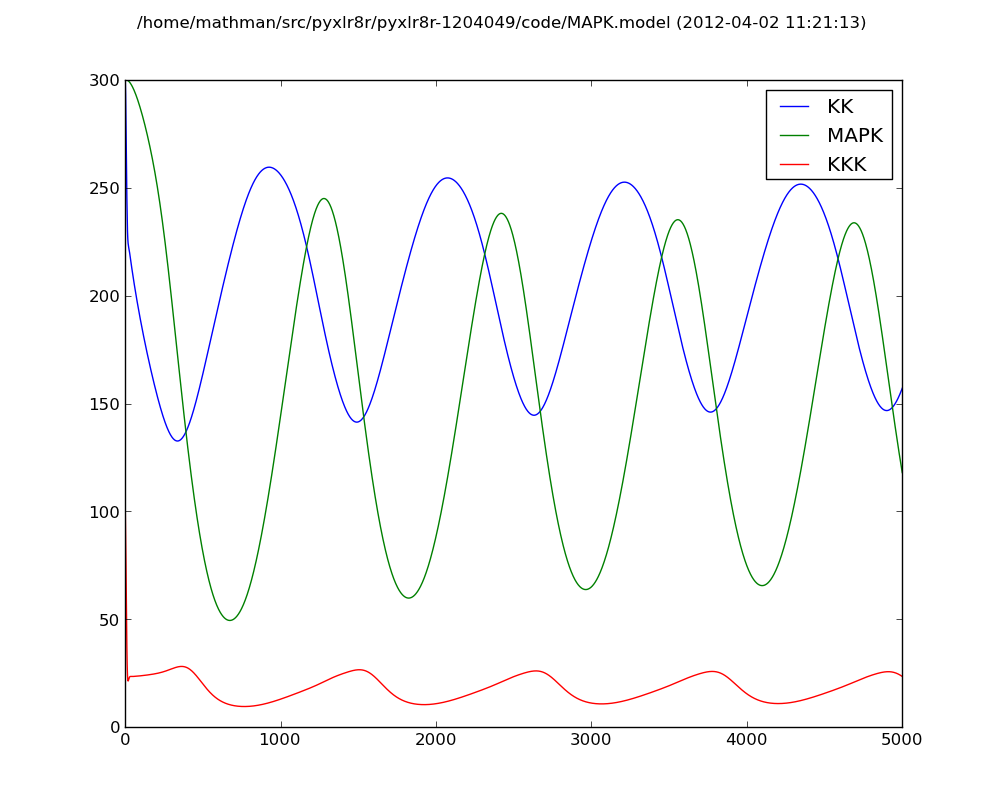
\includegraphics[width = .75\textwidth]{MAPK.png}
\end{center}

\section[Enzymes with Intermediate Complex]{Something That Illustrates Substrate/Enzyme and Product/Enzyme Complex Formation (TBD)} 

\section{Repressilator}
This model demonstrates the use of {\tt Hill} and {\tt rational} arrows.  An alternative version that uses {\tt USER} reactions is given at the end of this section.  A simulation model for the repressilator \cite{Repressilator} is given by\footnote{The terminating dollar sign at the end of the models is optional.}
\begin{center}
\begin{minipage}{4in}
\begin{scriptsize}
\begin{Verbatim}[frame=single]
$reactions
 [PX -> Nil, Beta]
 [PY -> Nil, Beta]
 [PZ -> Nil, Beta]
 [X -> X + PX, Beta]
 [Y -> Y + PY, Beta]
 [Z -> Z + PZ, Beta]
 [PZ |-> X, Hill[alpha1, n, K, 0, 1]]
 [PX |-> Y, Hill[alpha1, n, K, 0, 1]]
 [PY |-> Z, Hill[alpha1, n, K, 0, 1]]
 [X <-> Nil, rates[k1, alpha0]]
 [Y <-> Nil, rates[k1, alpha0]]
 [Z <-> Nil, rates[k1, alpha0]]
 [[[Nil],[PY]] ==> Z, rational[[alpha], [K, 1],[1], [n,n]]]
 [[[Nil],[PZ]] ==> X, rational[[alpha], [K, 1],[1], [n,n]]]
 [[[Nil],[PX]] ==> Y, rational[[alpha], [K, 1],[1], [n,n]]]
$rates
 alpha = 250
 alpha0 = 0
 alpha1 = 0
 Beta = 5
 n = 2.1 
 k1 = 1
 K = 1
$ic
 PX = 5
 PZ = 15
$
\end{Verbatim}
\end{scriptsize}
\end{minipage}
\end{center}
If we call this file {\tt repressilator.model} then the command\footnote{The leading dollar sign in the command refers to the bash prompt and should not be manually entered.}
\begin{center}
{\tt  \$ python solver.py -in repressilator.model -plot -run 100 .1}
\end{center}
will produce a plot such as this:
\begin{center}
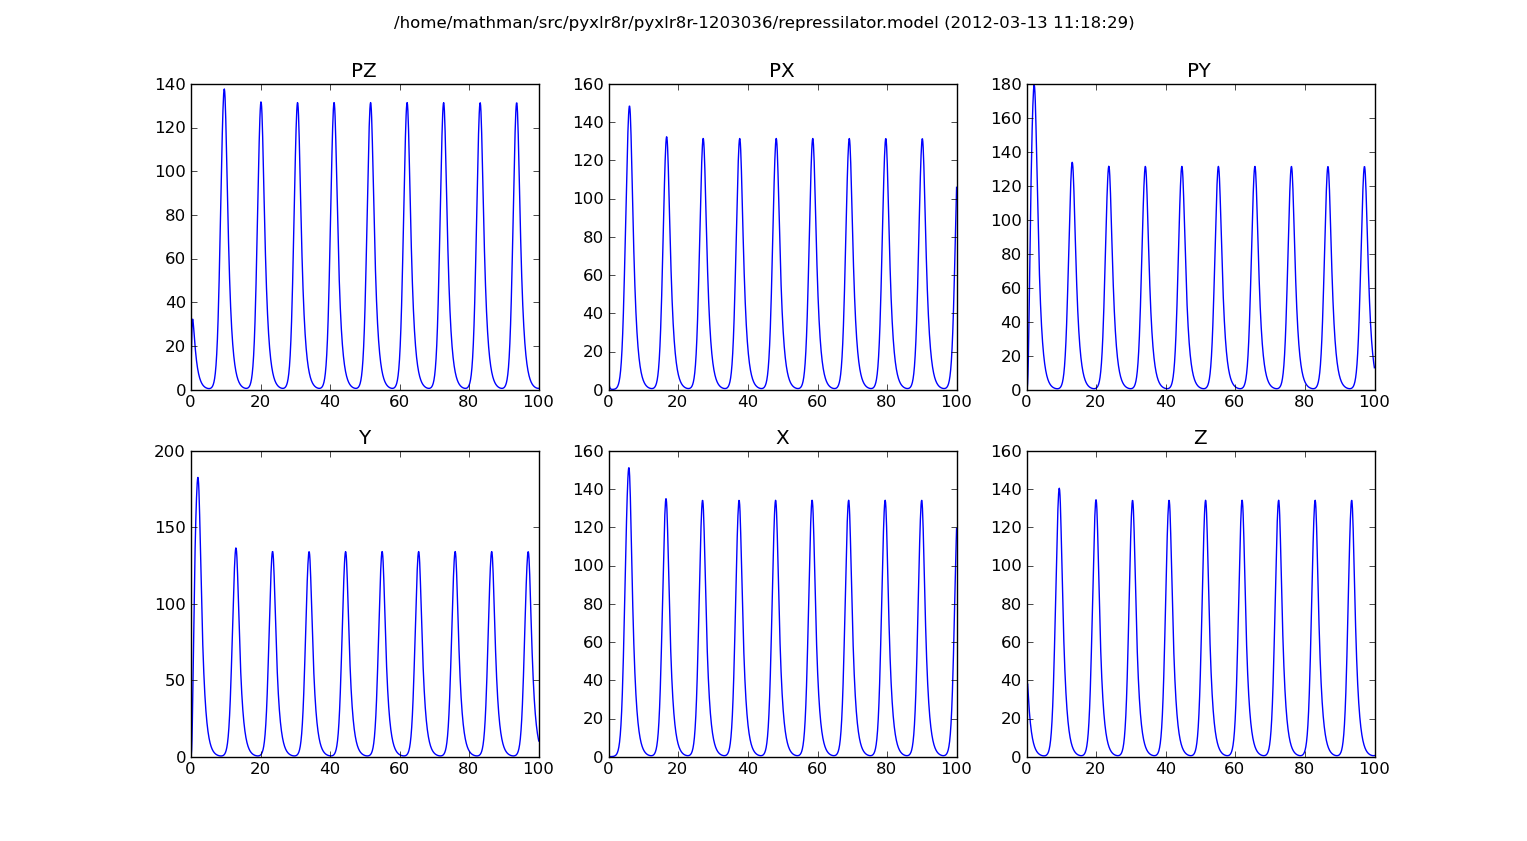
\includegraphics[width=.9\textwidth]{repressilator.png}
\end{center}
as well as a {\tt CSV} file that looks something like this:
\begin{center}
\begin{minipage}{5.5in}
\begin{scriptsize}
\begin{Verbatim}[frame=single]
0.0,15.0,5.0,0.0,0.0,0.0,0.0
0.1,14.2278260331,3.05384634588,0.247394702031,1.34912572721,0.0990958803047,23.562567514
0.2,21.504406326,1.90401628677,1.28225870666,4.57557848574,0.149799701424,37.9011356108
0.3,28.2774224855,1.21721312786,3.86093341284,11.2385014195,0.16314039654,38.2545583466
0.4,31.5798946122,0.803272174073,8.97682635583,22.2830086972,0.166187145597,35.2157392832
0.5,32.317811614,0.552727585611,17.2339097555,36.8646688505,0.166663798479,31.9877430887
...
99.8 0.648217893072,98.8724564077,14.3446430729,11.4817962739,113.312240676,0.649415887468
99.9,0.655884845799,105.886314242,12.9821534961,10.3905866114,119.451386878,0.685929274901
100.0,0.678921934741,112.385765424,11.7488271934,9.4030395272,124.765357623,0.74177680618
\end{Verbatim}
\end{scriptsize}
\end{minipage}
\end{center}
To see the differential equations produced by this model one could isolate the reactions in a file such as 
\begin{center}
\begin{minipage}{4in}
\begin{scriptsize}
\begin{Verbatim}[frame=single]
 [PX -> Nil, Beta]
 [PY -> Nil, Beta]
 [PZ -> Nil, Beta]
 [X -> X + PX, Beta]
 [Y -> Y + PY, Beta]
 [Z -> Z + PZ, Beta]
 [PZ |-> X, Hill[alpha1, n, K, 0, 1]]
 [PX |-> Y, Hill[alpha1, n, K, 0, 1]]
 [PY |-> Z, Hill[alpha1, n, K, 0, 1]]
 [X <-> Nil, rates[k1, alpha0]]
 [Y <-> Nil, rates[k1, alpha0]]
 [Z <-> Nil, rates[k1, alpha0]]
 [[[Nil],[PY]] ==> Z, rational[[alpha], [K, 1],[1], [n,n]]]
 [[[Nil],[PZ]] ==> X, rational[[alpha], [K, 1],[1], [n,n]]]
 [[[Nil],[PX]] ==> Y, rational[[alpha], [K, 1],[1], [n,n]]]
\end{Verbatim}
\end{scriptsize}
\end{minipage}
\end{center}
If we call this file {\tt repressilator.dat} then the command
\begin{center}
{\tt \$ python interpreter.py -in repressilator.dat}
\end{center}
will produce the output
\begin{center}
\begin{minipage}{4.5in}
\begin{scriptsize}
\begin{Verbatim}[frame=single]
PZ' = Beta*Z - Beta*PZ
PX' = Beta*X - Beta*PX
PY' = Beta*Y - Beta*PY
Y' = alpha0 - Y*k1 + alpha/(K**n + PX**n) + alpha1*PX**n/(K**n + PX**n)
X' = alpha0 - X*k1 + alpha/(K**n + PZ**n) + alpha1*PZ**n/(K**n + PZ**n)
Z' = alpha0 - Z*k1 + alpha/(K**n + PY**n) + alpha1*PY**n/(K**n + PY**n)
\end{Verbatim}
\end{scriptsize}
\end{minipage}
\end{center}

A second version of the repressilator, would replace the three {\tt rational} reactions 

\begin{Verbatim}[frame=single]
[[[Nil],[PY]] ==> Z, rational[[alpha], [K, 1],[1], [n,n]]]
[[[Nil],[PZ]] ==> X, rational[[alpha], [K, 1],[1], [n,n]]]
[[[Nil],[PX]] ==> Y, rational[[alpha], [K, 1],[1], [n,n]]]
\end{Verbatim}

with the three {\tt USER} reactions to generate the same identical differential equations:

\begin{Verbatim}[frame=single]
[PY |-> Z, USER[alpha, -1, n, 0, "lambda x: 1/(K**n+x)"]]
[PZ |-> X, USER[alpha, -1, n, 0, "lambda x: 1/(K**n+x)"]]
[PX |-> Y, USER[alpha, -1, n, 0, "lambda x: 1/(K**n+x)"]]
\end{Verbatim}

\newpage
\section{Lineage Determination}

This model demonstrates the use of the rational with product notation. The model is based on \cite{Chickarmane}. 
\begin{multicols}{2}
\begin{tiny}
\begin{Verbatim}[frame=single]
$REACTIONS
 [[[A,O*S,O*S*N],[A, O,O*S,O*S*N,C*O,GC]]==>O, rational[[a0,a1,a2,a3],
     [1,b0,b1,b2,b3,b4,b5], [],[]]]
 [O->Nil,gamma1]
#
 [[[O*S, O*S*N], [O, O*S, O*S*N]] ==>S, rational[[c0,c1,c2],
     [1,d0,d1,d2],[],[]]]
 [S->Nil,gamma2]
#
 [[[O*S,O*S*N],[O,O*S,O*S*N,O*G]] ==>N, rational[[e0,e1,e2],
    [1,f0,f1,f2,f3],[],[]]]
 [N->Nil,gamma3]
#
 [[[C],[C,C*O]]==>C, rational[[g0,g1],[1,h0,h1],[],[]]]
 [C->Nil,gamma4]
#
 [[[C,G],[C,G]]==>GC, rational[[i0,i1,i2],[1,j0,j1],[],[]]]
 [GC->Nil,gamma5]
#
 [[[O,G],[O,G,N]]==>G, rational[[p0,p1,p2],[1,q0,q1,q2],[],[]]]
 [G->Nil, gammag]
#
 [A->A,1]
$IC
 O=5
 N=5
 S=5
 G=0
 GC=0
 C=0
 A=1
$Rates
a0 = 0.001
 a1 = 1
 a2 = 0.005
 a3 = 0.025
 b0 = 1
 b1 = 0.001
 b2 = 0.005
 b3 = 0.025
 b4 = 10
 b5 = 10
 gamma1 = 0.1
 c0 = 0.001
 c1 = 0.005
 c2 = 0.025
 d0 = 0.001
 d1 = 0.005
 d2 = 0.025
 gamma2 = 0.1
 e0 = 0.001
 e1 = 0.1
 e2 = 0.1
 f0 = 0.001
 f1 = 0.1
 f2 = 0.1
 f3 = 10
 gamma3 = 0.1
 g0 = 0.001
 g1 = 2
 h0 = 2
 h1 = 5
 gamma4 = 0.1
 gamma5 = 0.1
 i0 = 0.001
 i1 = 0.1
 i2 = 0.1
 j0 = 0.1
 j1 = 0.1
 p0 = 0.1
 p1 = 1.
 p2 = 0.00025
 q0 = 1.
 q1 = 0.00025
 q2 = 15
 gammag = 0.1
$ 
\end{Verbatim}
\end{tiny}
\end{multicols}
\begin{verbatim}
      python pyx.py solve -in CP.model -plot -run 300 1 -sameplot
\end{verbatim}
\begin{center}
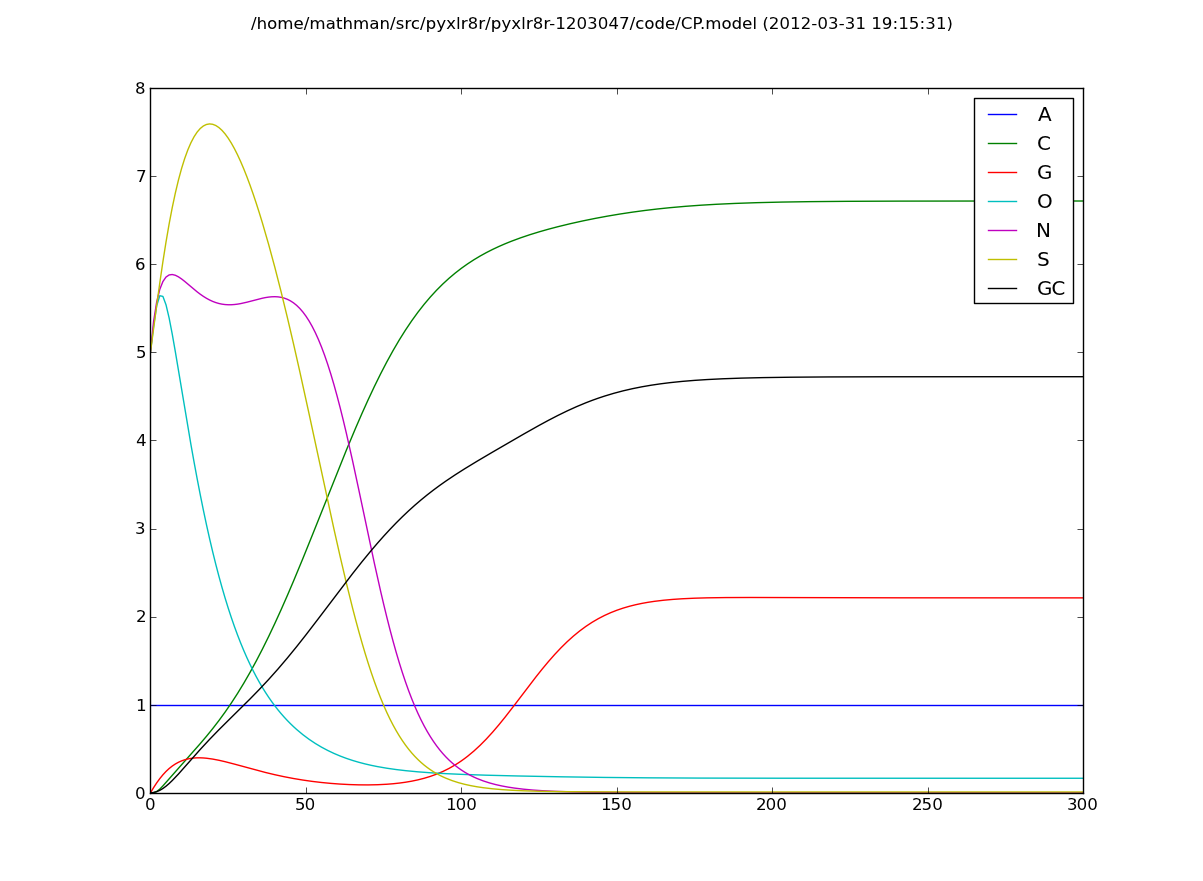
\includegraphics[width=.75\textwidth]{chickarmane.png}
\end{center}

\newpage

\section{NF-$\kappa\beta$ Signaling Model}

A pycellerator model of the the  NF-$\kappa\beta$ signaling model of \cite{NFKB} is given by:

\begin{changemargin}{1.5in}{1in}
%\begin{center}
%\begin{minipage}{4.5in}
\begin{scriptsize}
\begin{Verbatim}[frame=single,xrightmargin=\leftmargin]
$Reactions
 [IkBa + NFkB <-> IkBa_NFkB, rates[a1, d1]]
 [IKK_IkBa + NFkB <-> IKK_IkBa_NFkB, rates[a2, d2]]
 [NFkB <-> NFkBn, rates[tr1, tr2]]
 [IkBa_NFkB -> NFkB, deg1]
 [IkBan + NFkBn <-> IkBan_NFkBn, rates[a1, d1]] 
 [IkBa + IKK <-> IKK_IkBa, rates[a3, d3]]
 [IkBat -> Nil, deg3]
 [IkBa <-> IkBan, rates[tr3, tr4]]
 [IKK_IkBa_NFkB -> IKK + NFkB, k1] 
 [IKK_IkBa -> IKK, k2]
 [IkBat |-> IkBa, Hill[v1, n1, K1]]
 [IkBa_NFkB <-> IkBan_NFkBn, rates[tr5, tr6]]
 [IkBa -> Nil, deg2]
 [NFkBn |-> IkBat, Hill[v2, n2, K2]] 
 [Nil -> IkBat, trb]
 [IkBa_NFkB + IKK <-> IKK_IkBa_NFkB, rates[a4, d4]] 
 [IKK -> Nil, adapt]
$IC
 NFkB = 0.003053
 IkBa = 0.372
 IkBa_NFkB = 0.09826
 NFkBn = .00047638
 IkBan = 0.11937
 IkBan_NFkBn = 0.001985
 IKK = 0.1
 IkBat = 0.008454217
 IKK_IkBa_NFkB = 0
 IKK_IkBa = 0
$Rates
 v1 = 2.448
 K1 = 10
 n1 = 1
 v2 = 1.02713
 K2 = 1
 n2 = 2
 a1 =  30 
 a2= 30
 a3= 1.35
 a4= 11.1
 tr1= 5.4 
 tr2= 0.0048
 tr3= 0.018
 tr4= 0.012
 tr5= 0
 tr6= 0.82944
 d1= 0.03 
 d2= 0.03
 d3= 0.0075
 d4= 0.105
 deg1= 0.00135 
 deg2= 0.00675 
 deg3= 0.0168
 k1= 1.221
 k2= 0.2442 
 trb=0.0000921375
 adapt= 0.0072
$
\end{Verbatim}
\end{scriptsize}
%\end{minipage}
%\end{center}
\end{changemargin}

Running a simulation with this file as {\tt NFKB.model} using the command
\begin{center}
{\tt  python solver.py -in NFKB.model -plot IKK IkBa NFkB -run 500 .1}
\end{center}


will produce the following plot:
\begin{center}
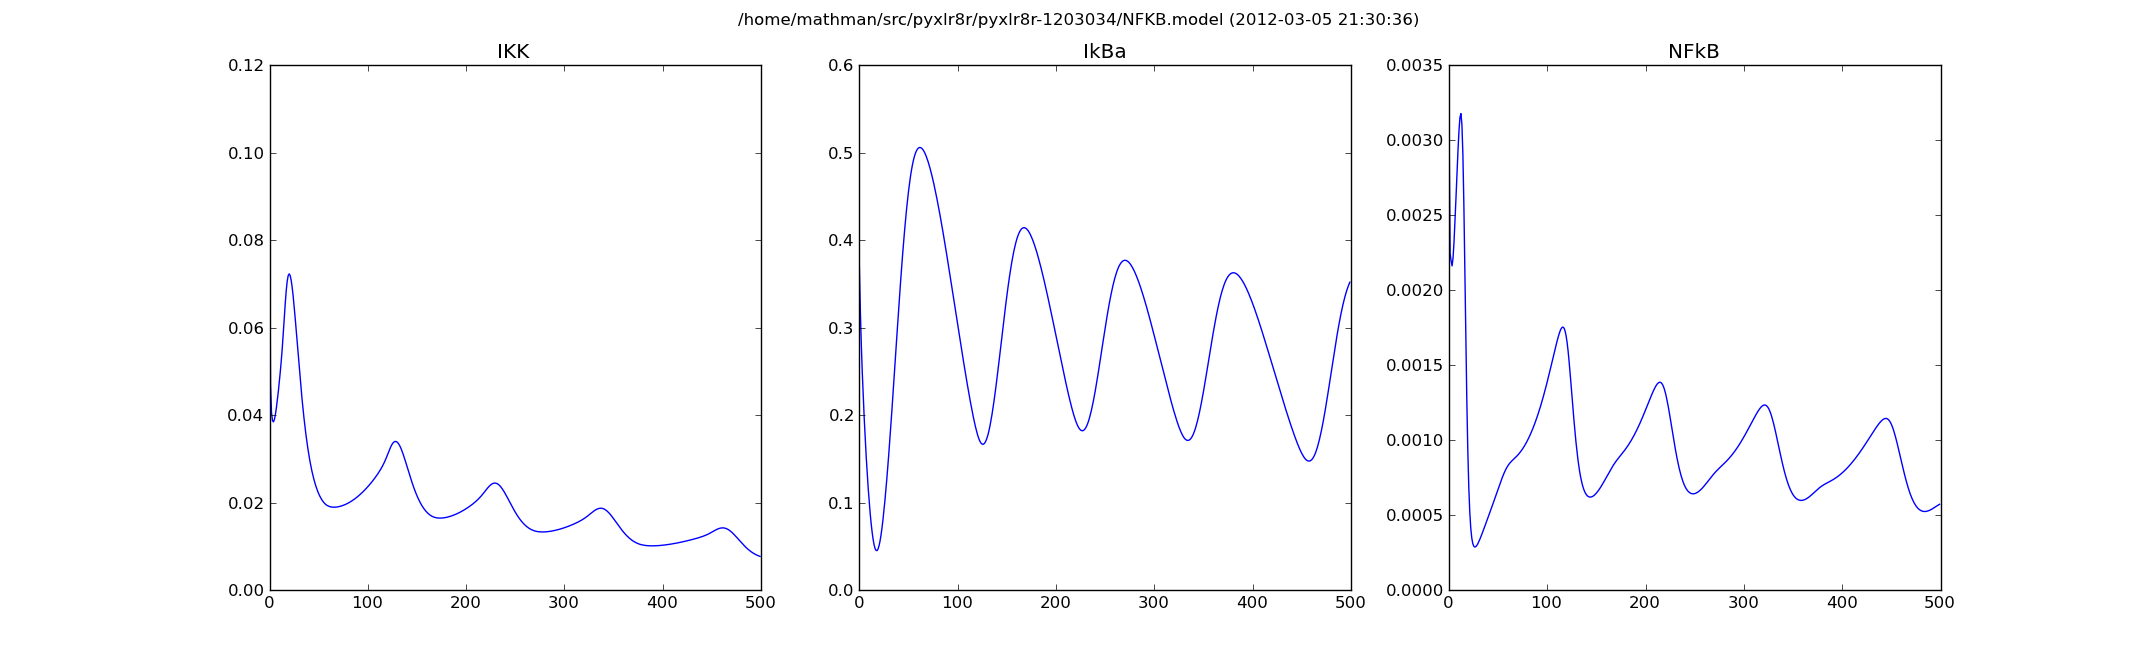
\includegraphics[width=\textwidth]{NFKB.png}
\end{center}

The differential equations produced from the file {\tt NFKB.dat}:
\begin{changemargin}{1.5in}{1in}
\begin{scriptsize}
\begin{Verbatim}[frame=single,xrightmargin=\leftmargin]
 [IkBa + NFkB <-> IkBa_NFkB, rates[a1, d1]]
 [IKK_IkBa + NFkB <-> IKK_IkBa_NFkB, rates[a2, d2]]
 [NFkB <-> NFkBn, rates[tr1, tr2]]
 [IkBa_NFkB -> NFkB, deg1]
 [IkBan + NFkBn <-> IkBan_NFkBn, rates[a1, d1]] 
 [IkBa + IKK <-> IKK_IkBa, rates[a3, d3]]
 [IkBat -> Nil, deg3]
 [IkBa <-> IkBan, rates[tr3, tr4]]
 [IKK_IkBa_NFkB -> IKK + NFkB, k1] 
 [IKK_IkBa -> IKK, k2]
 [IkBat |-> IkBa, Hill[v1, n1, K1]]
 [IkBa_NFkB <-> IkBan_NFkBn, rates[tr5, tr6]]
 [IkBa -> Nil, deg2]
 [NFkBn |-> IkBat, Hill[v2, n2, K2]] 
 [Nil -> IkBat, trb]
 [IkBa_NFkB + IKK <-> IKK_IkBa_NFkB, rates[a4, d4]] 
 [IKK -> Nil, adapt]
\end{Verbatim}
\end{scriptsize}
\end{changemargin}
are obtained via
\begin{center}
{\tt python interpreter.py -in NFKB.dat}
\end{center}
and look like this:
\begin{changemargin}{0.2in}{1in}
\begin{scriptsize}
\begin{Verbatim}[frame=single,xrightmargin=\leftmargin]
IkBa_NFkB' = IKK_IkBa_NFkB*d4 + IkBan_NFkBn*tr6 - IkBa_NFkB*d1 - IkBa_NFkB*deg1 - IkBa_NFkB*tr5 +
  IkBa*NFkB*a1 - IKK*IkBa_NFkB*a4
IkBan_NFkBn' = IkBa_NFkB*tr5 - IkBan_NFkBn*d1 - IkBan_NFkBn*tr6 + IkBan*NFkBn*a1
IKK_IkBa' = IKK_IkBa_NFkB*d2 - IKK_IkBa*d3 - IKK_IkBa*k2 + IKK*IkBa*a3 - IKK_IkBa*NFkB*a2
NFkBn' = IkBan_NFkBn*d1 + NFkB*tr1 - NFkBn*tr2 - IkBan*NFkBn*a1
IKK_IkBa_NFkB' = -IKK_IkBa_NFkB*d2 - IKK_IkBa_NFkB*d4 - IKK_IkBa_NFkB*k1 + IKK*IkBa_NFkB*a4 + 
 IKK_IkBa*NFkB*a2
NFkB' = IKK_IkBa_NFkB*d2 + IKK_IkBa_NFkB*k1 + IkBa_NFkB*d1 + IkBa_NFkB*deg1 + NFkBn*tr2 - NFkB*tr1 -
 IKK_IkBa*NFkB*a2 - IkBa*NFkB*a1
IkBan' = IkBa*tr3 + IkBan_NFkBn*d1 - IkBan*tr4 - IkBan*NFkBn*a1
IkBa' = IKK_IkBa*d3 + IkBa_NFkB*d1 + IkBan*tr4 - IkBa*deg2 - IkBa*tr3 - IKK*IkBa*a3 - IkBa*NFkB*a1 +
 v1*IkBat**n1/(IkBat**n1 + K1**n1)
IkBat' = trb - IkBat*deg3 + v2*NFkBn**n2/(K2**n2 + NFkBn**n2)
IKK' = IKK_IkBa*d3 + IKK_IkBa*k2 + IKK_IkBa_NFkB*d4 + IKK_IkBa_NFkB*k1 - IKK*adapt - IKK*IkBa*a3 -
 IKK*IkBa_NFkB*a4
\end{Verbatim}
\end{scriptsize}
\end{changemargin}
If the {\tt code} option is requested, e.g., 
\begin{center}
{\tt python interpreter.py -in NFKB.dat -format CODE -out nfkb.py}
\end{center}
The the file {\tt nfkb.py} will look something like this:\footnote{While each line of code terminates with a newline character, individual lines of code are not line-wrapped and may be very line. The wrapping shown here was edited for illustration in this document, so in fact, it is likely that most lines of code will exceed the standard 80 character page width. This is why the usual python line wrap characters are not shown in the example.}

\begin{changemargin}{0.3in}{1in}
\begin{scriptsize}
\begin{Verbatim}[frame=single,xrightmargin=\leftmargin]
def f(y,t):
    y[0] = IkBa_NFkB
    y[1] = IkBan_NFkBn
    y[2] = IKK_IkBa
    y[3] = NFkBn
    y[4] = IKK_IkBa_NFkB
    y[5] = NFkB
    y[6] = IkBan
    y[7] = IkBa
    y[8] = IkBat
    y[9] = IKK
    yp[0] = IKK_IkBa_NFkB*d4 + IkBan_NFkBn*tr6 - IkBa_NFkB*d1 - 
    	IkBa_NFkB*deg1 - IkBa_NFkB*tr5 + IkBa*NFkB*a1 - IKK*IkBa_NFkB*a4
    yp[1] = IkBa_NFkB*tr5 - IkBan_NFkBn*d1 - IkBan_NFkBn*tr6 + IkBan*NFkBn*a1
    yp[2] = IKK_IkBa_NFkB*d2 - IKK_IkBa*d3 - IKK_IkBa*k2 + IKK*IkBa*a3 
    	- IKK_IkBa*NFkB*a2
    yp[3] = IkBan_NFkBn*d1 + NFkB*tr1 - NFkBn*tr2 - IkBan*NFkBn*a1
    yp[4] = -IKK_IkBa_NFkB*d2 - IKK_IkBa_NFkB*d4 - IKK_IkBa_NFkB*k1 + IKK*IkBa_NFkB*a4 
    	+ IKK_IkBa*NFkB*a2
    yp[5] = IKK_IkBa_NFkB*d2 + IKK_IkBa_NFkB*k1 + IkBa_NFkB*d1 + IkBa_NFkB*deg1 + NFkBn*tr2 
    	- NFkB*tr1 - IKK_IkBa*NFkB*a2 - IkBa*NFkB*a1
    yp[6] = IkBa*tr3 + IkBan_NFkBn*d1 - IkBan*tr4 - IkBan*NFkBn*a1
    yp[7] = IKK_IkBa*d3 + IkBa_NFkB*d1 + IkBan*tr4 - IkBa*deg2 - IkBa*tr3 - IKK*IkBa*a3 
    	- IkBa*NFkB*a1 + v1*IkBat**n1/(IkBat**n1 + K1**n1)
    yp[8] = trb - IkBat*deg3 + v2*NFkBn**n2/(K2**n2 + NFkBn**n2)
    yp[9] = IKK_IkBa*d3 + IKK_IkBa*k2 + IKK_IkBa_NFkB*d4 + IKK_IkBa_NFkB*k1 - IKK*adapt 
    	- IKK*IkBa*a3 - IKK*IkBa_NFkB*a4
    return (yp)
\end{Verbatim}
\end{scriptsize}
\end{changemargin}

\pagebreak
\section{Minimal Mitotic Model}
\label{section:Goldbeter}

This is a standard minimal model of a mitotic oscillator\cite{Goldbeter}. It illustrates the use non-catalytic Hill function arrows as well as the use of equations as part of the rate constants. The model is given by:
\begin{tiny}
\begin{Verbatim}[frame=single]
# Goldbeter, A. A minimal cascade model for the mitotic
# oscillator involving cyclin and cdc2 kinase. Proc. Natl.
# Acad. Sci. USA 88:9107-1101 (1991).
$REACTIONS
 [C <-> Nil, rates[kd, vi]]
 [C |--> Nil, mod[X], Hill[vd, 1, Kd, 0,1 ]]
 [M |--> Nil, mod[Nil], Hill[v2, 1, K2, 0, 1]]
 [X |--> Nil, mod[Nil], Hill[v4, 1, K4, 0, 1]]
 [Nil -> X, " vm3 * M * (1-X)/(K3+1-X)"]
 [C |-> M, Hill[" vm1*(1-M)/(K1+1-M)", 1, Kc, 0, 1]]
$IC
 C = 0.1
 M = 0.2
 X = 0.3
$RATES
 vd = 0.1
 vi = 0.023
 v2 = 0.167
 v4 = 0.1
 vm1 = 0.5
 vm3 = 0.2
 kd = 0.00333
 K1 = 0.1
 K2 = 0.1
 K3 = 0.1
 K4 = 0.1
 Kc = 0.3
 Kd = 0.02
$
\end{Verbatim}
\end{tiny}
\begin{verbatim}
  $  python pyx.py solve -in Goldbeter.model  -plot -run 100 .1 -sameplot
\end{verbatim}
\begin{center}
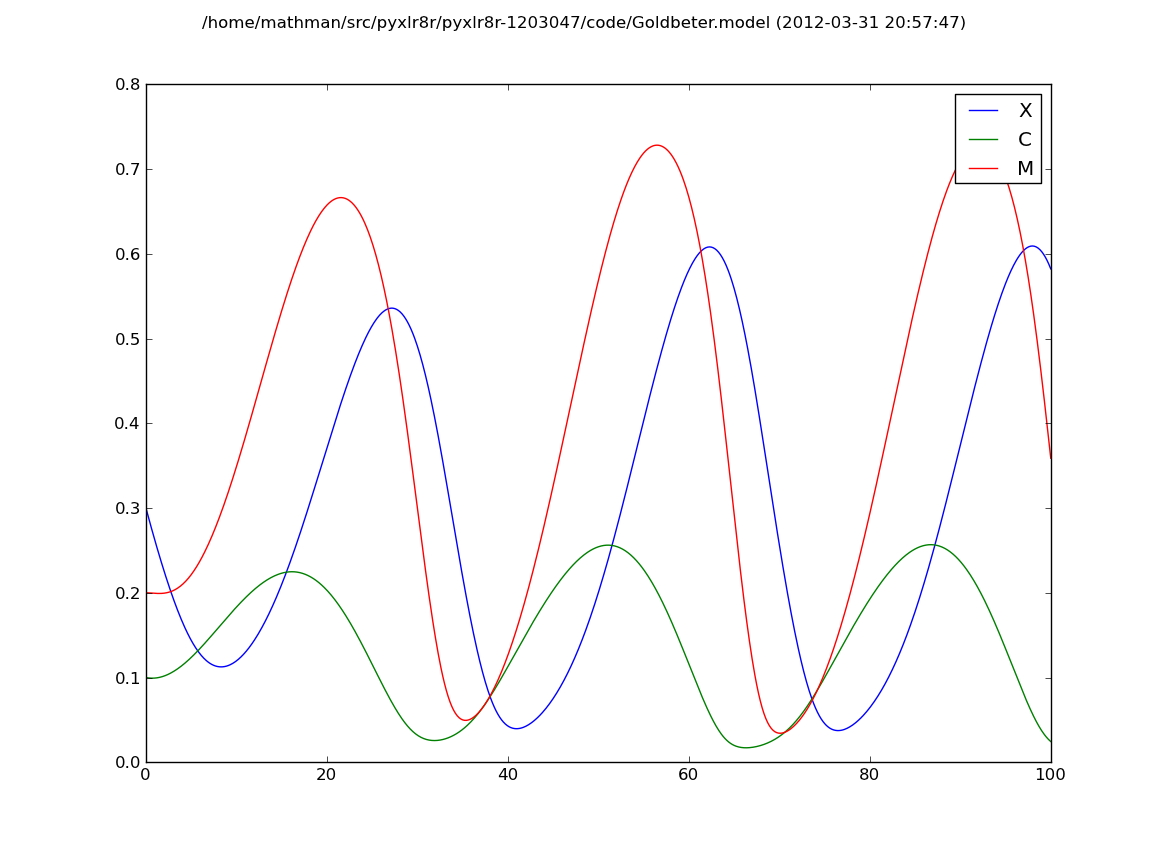
\includegraphics[width=.85\textwidth]{Goldbeter.png}
\end{center}

\pagebreak

\section[Ring Oscillator (Mass Action)]{Ring Oscillator Using Mass Action Equations}

The following model describes a ring oscillator using only mass-action equations: 
\begin{changemargin}{1.5in}{1in}
\begin{scriptsize}
\begin{Verbatim}[frame=single,xrightmargin=\leftmargin]
$Reactions
 [X  <=> XP,   mod[Z, ZPP], rates[a, d, k, 0,  a, d, k]]
 [XP <=> XPP,  mod[Z, ZPP], rates[a, d, k, 0, a, d, k]]
 [Y  <=> YP,   mod[X, XPP], rates[a, d, k, 0, a, d, k]] 
 [YP <=> YPP,  mod[X, XPP], rates[a, d, k, 0, a, d, k]] 
 [Z  <=> ZP,   mod[Y, YPP], rates[a, d, k, 0, a, d, k]]
 [ZP <=> ZPP,  mod[Y, YPP], rates[a, d, k, 0, a, d, k]]
$IC
 X = 10.0
 Y = 15.0
 Z = 20.0
$Rates
 a = 1.0
 d = 1.0
 k = 1.0
$
\end{Verbatim}
\end{scriptsize}
\end{changemargin}

\begin{center}
{\tt  python solver.py -in ringma.model -plot -run 100 .1 -plotcolumns 1}
\end{center}

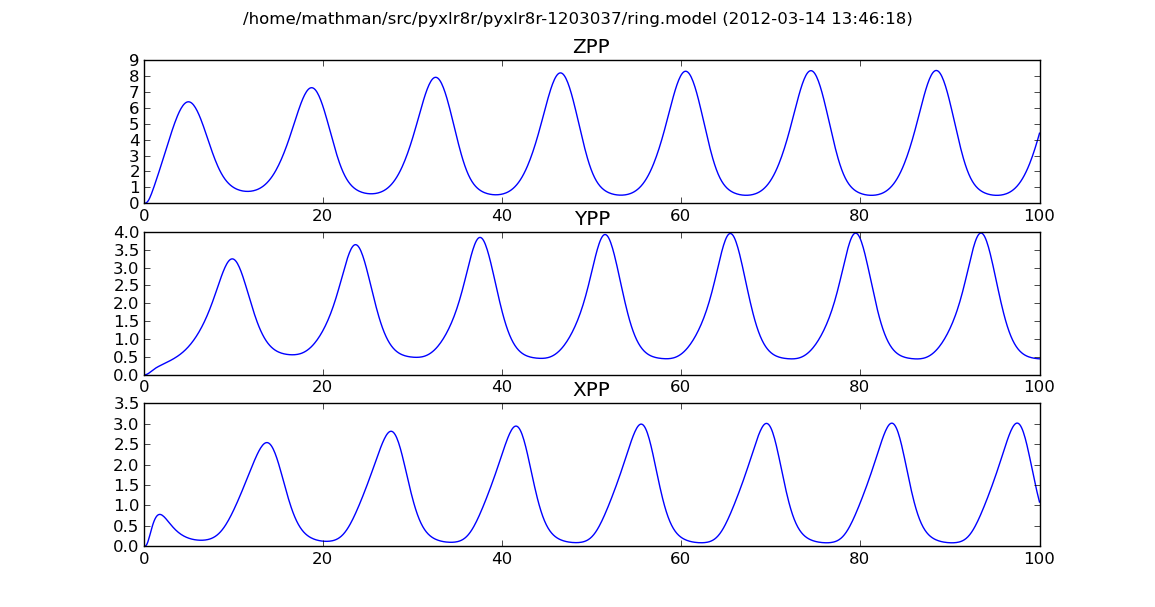
\includegraphics[width=\textwidth]{ringma.png}

\pagebreak

%\section{Something That Illustrates MMH alternate form (TBD)} 

\section[Ring Oscillator (MMH)]{Ring Oscillator Using Michaelis-Menten-Henri Reactions}


\begin{changemargin}{1.5in}{1in}
\begin{scriptsize}
\begin{Verbatim}[frame=single,xrightmargin=\leftmargin]
$Reactions
 [X :--> XP, mod[Z], MMH[K,v]]
 [XP:--> X,  mod[ZP],MMH[K,v]]
 [Y :--> YP, mod[X], MMH[K,v]]
 [YP:--> Y,  mod[XP],MMH[K,v]]
 [Z :--> ZP, mod[Y], MMH[K,v]]
 [ZP:--> Z,  mod[YP],MMH[K,v]]
$IC
 X = 1.0
 Y = 2.0
 Z = 3.0
$Rates
 v=1.0
 K=0.5
$
\end{Verbatim}
\end{scriptsize}
\end{changemargin}

\begin{center}
{\tt  python solver.py -in ringmm.model -plot -run 25 .1 -plotcolumns 1}
\end{center}

\begin{center}
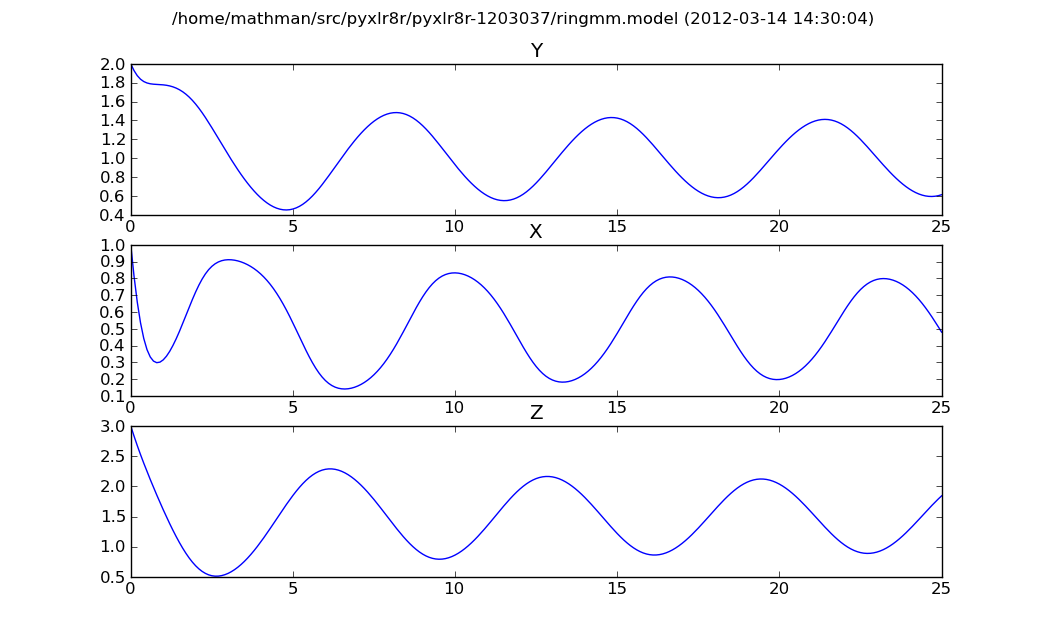
\includegraphics[width=\textwidth]{ringmm.png}
\end{center}

\pagebreak

%\section{GRN Multiple Substrates (TBD)}

\section{Ring Oscillator Using GRN Reactions}

\begin{changemargin}{1.5in}{1in}
\begin{scriptsize}
\begin{Verbatim}[frame=single,xrightmargin=\leftmargin]
$Reactions
 [U |-> V, GRN[v, b, n, h]]
 [V |-> W, GRN[v, b, n, h]]
 [W |-> U, GRN[v, b, n, h]]
 [V -> Nil, k]
 [U -> Nil, k]
 [W -> Nil, k]
$IC
 U = .5
 V = .4
 W = 0.6
$Rates
 v = 1
 n = 2
 h = 1
 k = 0.5
 b = -10
$
\end{Verbatim}
\end{scriptsize}
\end{changemargin}

\begin{center}
{\tt  python solver.py -in ringgrn.model -plot -run 50 .1 -sameplot}
\end{center}

\begin{center}
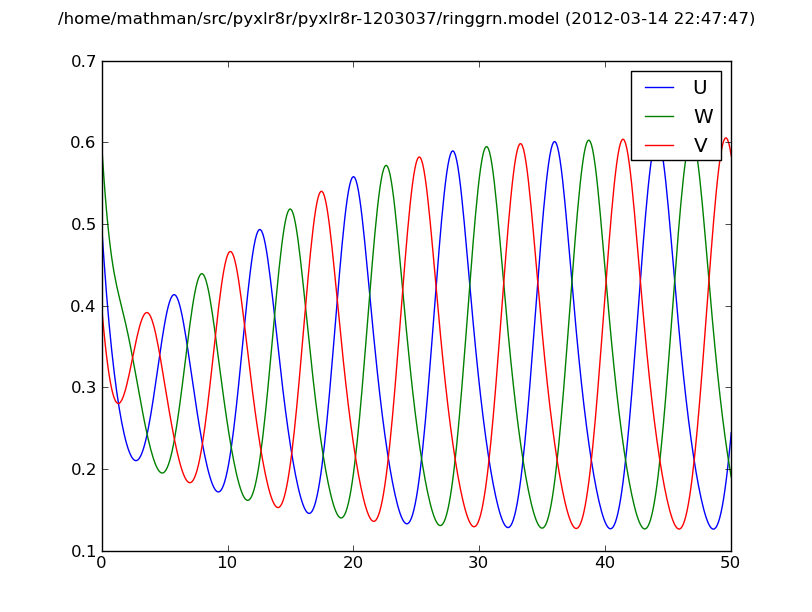
\includegraphics[width=.7\textwidth]{ringgrn.png}
\end{center}

\pagebreak
%\section{Something That Illustrates NHCA Multiple Substrates(TBD)}

\section[Ring Oscillator (NHCA)]{Ring Oscillator Using NHCA Reactions}

\begin{changemargin}{1.5in}{1in}
\begin{scriptsize}
\begin{Verbatim}[frame=single,xrightmargin=\leftmargin]
$Reactions
 [U |-> V, NHCA[v,TP,TM,n,m,K]]
 [V |-> W, NHCA[v,TP,TM,n,m,K]]
 [W |-> U, NHCA[v,TP,TM,n,m,K]]
 [V -> Nil, k]
 [U -> Nil, k]
 [W -> Nil, k]
$IC
 U = .6
 V = .75
 W = .5
$Rates
 v = 1
 n = 2
 m = 2
 K = 10
 k = 1
 TP=.2
 TM=-5
$
\end{Verbatim}
\end{scriptsize}
\end{changemargin}

\begin{center}
{\tt  python solver.py -in ringnhca.model -plot -run 25 .1 -sameplot}
\end{center}

\begin{center}
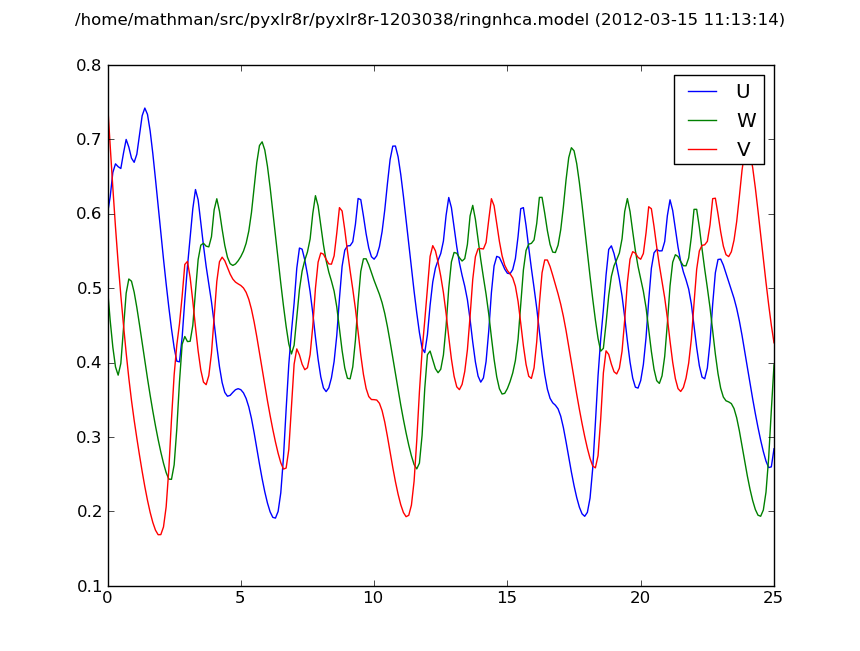
\includegraphics[width=.7\textwidth]{ringnhca.png}
\end{center}

\section{Recombinant \textit{E coli} growth model}

This model uses an S-System approach that is given by \cite{ecoli}.

\begin{changemargin}{1.25in}{1in}
\begin{scriptsize}
\begin{Verbatim}[frame=single,xrightmargin=\leftmargin]
$reactions
[[X1,X2] |-> X1,    SSystem[1, a1, b1, [g11,g12], [h11,h12]]]
[[X1,X2] |-> X2,    SSystem[1, a2, b2, [0, 0], [h21, h22]]]
[[X1,X2,X3] |-> X3, SSystem[1, a3, b3, [g31,g32,0], [h31,h32,h33]]]
[[X1,X2,X4] |-> X4, SSystem[1, a4, b4, [g41,g42,0], [h41,h42,h44]]]
[[X1,X2,X5] |-> X5, SSystem[1, a5, b5, [g51,g52,0], [h51,h52,h55]]]
$ic
X1 = 0.1
X2 = 10
X3 = 0.1
X4 = 0.1
X5 = 0.1
$rates
a1 = 0.4973
a2 = 0.0817
a3 = 0.2858
a4 = 3.7124
a5 = 0.4562
b1 = 0.1648
b2 = 1.2484
b3 = 0.1285
b4 = 2.5318
b5 = 0.0335
g11 = 0.9099
g31 = 0.7366
g41 = 1.7076
g51 = 0.2292
g12 = 0.1301
g32 = 0.1311
g42 = 0.1252
g52 = 0.0277
h11 = 1.7514
h21 = 0.9325
h31 = 1.3535
h41 = 1.9875
h51 = 1.1978
h12 = 0.1292
h22 = 0.1927
h32 = 0.1175
h42 = 0.1210
h52 = 0.4462
h33 = -0.0110
h44 = -0.0100
h55 = -0.0426
$
\end{Verbatim}
\end{scriptsize}
\end{changemargin}


\begin{center}
{\tt  python solver.py -in ecoli.model -plot -run 24 .1 -sameplot}
\end{center}

\begin{center}
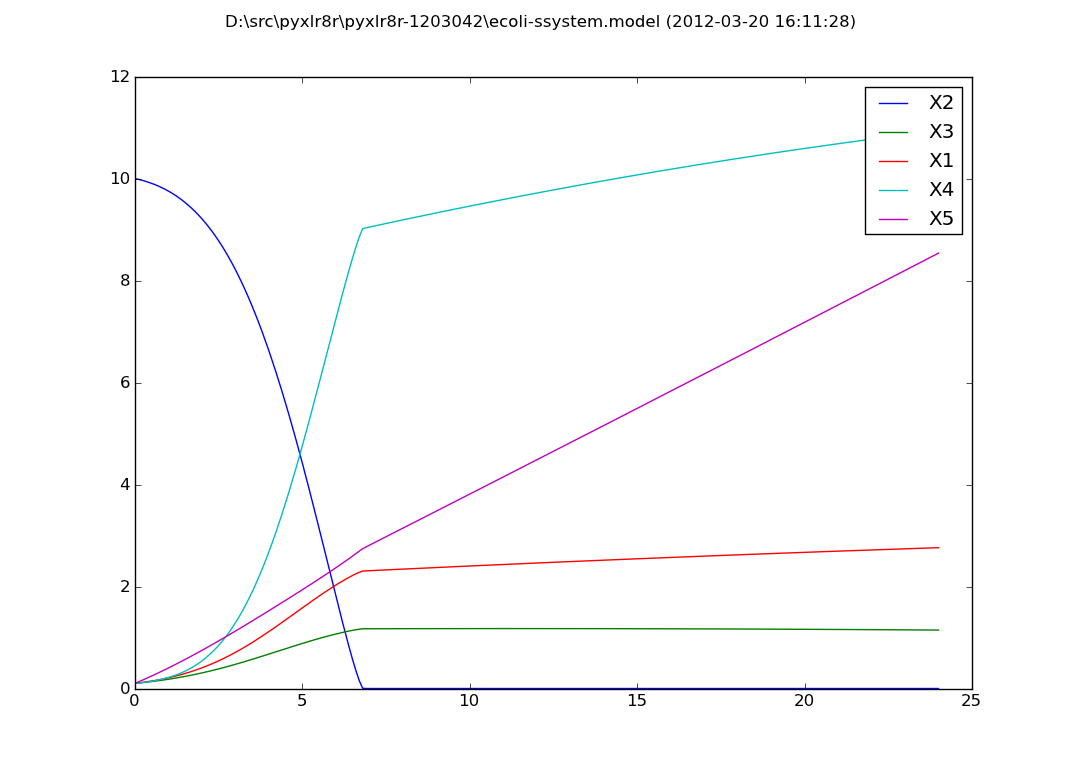
\includegraphics[width=.7\textwidth]{ecoli-ssystem.png}
\end{center}


\section[Monow-Wyman-Changeaux (MWC)]{Something That Illustrates MWC (TBD)}

\section{MAPK Cascade with Indexed Stages}

\begin{multicols}{2}
\begin{tiny}
\begin{Verbatim}[frame=single]
$Reactions
 [K(3,0) <=> K(3,1), mod[RAFK, RAFph], rates[a1,d1,k1,0,a2,d2,k2,0]]
 [K(2,0) <=> K(2,1) <=> K(2,2), mod[ K(3,1), MEKph ], rates[ a3, d3, k3, 0, a4, d4, k4, 0, a5, d5, k5, 0, a6, d6, k6, 0]]
 [K(1,0) <=> K(1,1) <=> K(1,2), mod[ K(2,2), MAPKph ], rates[ a7, d7, k7, 0, a8, d8, k8, 0, a9, d9, k9, 0, a10, d10, k10, 0]]
$IC
 K(3,0) = 1
 K(2,0) = 2.5
 K(1,0) = 1.7
 RAFK = 1
$Rates
 a1=1.
 a2=0.5
 a3=3.3
 a4=10.
 a5=3.3
 a6=10.
 a7=20.
 a8=5.
 a9=20.
 a10=5.
 d1=.4
 d2=.5
 d3=.42
 d4=.8
 d5=.4
 d6=.8
 d7=.6
 d8=.4
 d9=.6
 d10=.4
 k1=.1
 k2=.1
 k3=.1
 k4=.1
 k5=.1
 k6=.1
 k7=.1
 k8=.1
 k9=.1
 k10=.1
$
\end{Verbatim}
\end{tiny}
\end{multicols}

{\tt \$ python pyx.py solve -in MAPK-Indexed.model -solve -plot K(1,0) \\
 \hspace{.5in} K(1,1) K(1,2) K(2,0) K(2,1) K(2,2) K(3,0) K(3,1) -sameplot }
 
\begin{center}
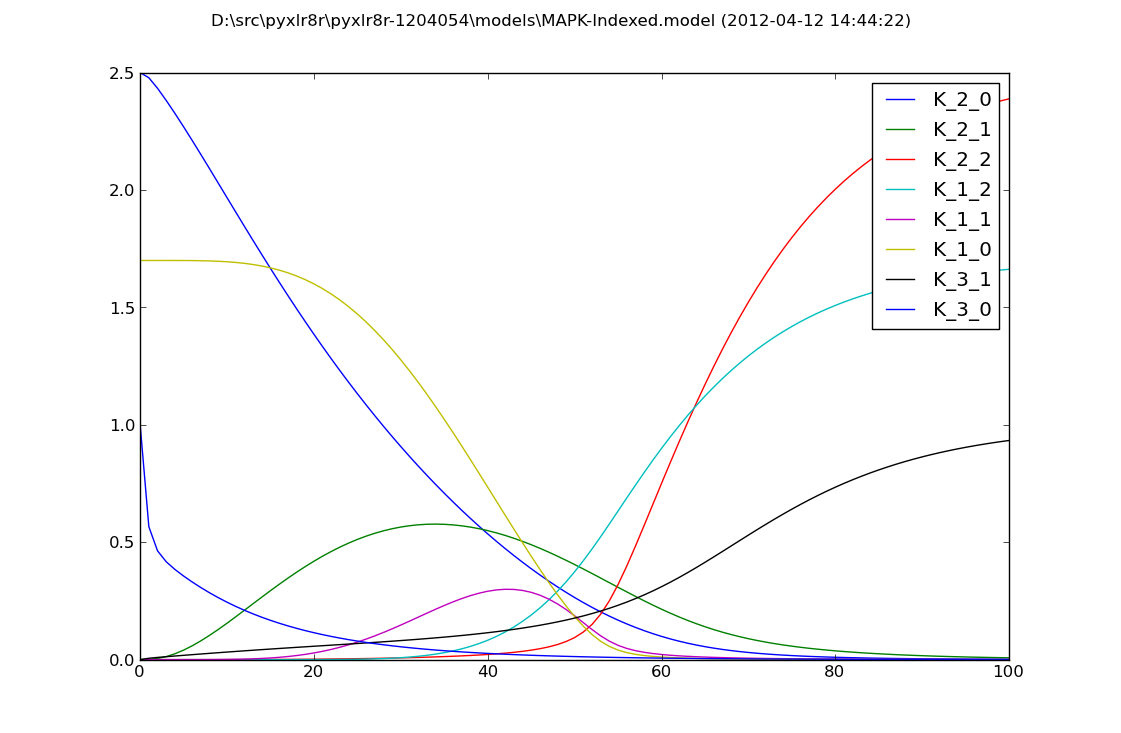
\includegraphics[width=.75\textwidth]{MAPK-Indexed.png}
\end{center}